\documentclass{beamer}
\usetheme{Madrid}
\usepackage[T1]{fontenc}
\usepackage{mathpazo}
\usepackage{graphicx}
\usepackage{booktabs}
\usepackage{tikz}
\usetikzlibrary{positioning,arrows.meta,shapes.geometric,fit,backgrounds,calc}
\definecolor{cetnavy}{RGB}{10,26,63}
\definecolor{cetlight}{RGB}{225,231,242}
\setbeamercolor{structure}{fg=cetnavy}
\setbeamercolor{frametitle}{bg=cetnavy,fg=white}
\setbeamercolor{title}{bg=cetnavy,fg=white}
\setbeamertemplate{navigation symbols}{}
% =====================================================================
%  EDIT YOUR DETAILS HERE — this ONE file feeds every abstract & deck.
%  (Change a value, recompile; all 36 documents update.)
% =====================================================================
\newcommand{\seminarName}{Aflah Muhammed P}      % <-- your full name (guessed from your email; please verify)
\newcommand{\seminarRoll}{TVE00CS000}            % <-- your university register/roll number
\newcommand{\seminarClassRoll}{00}               % <-- your class roll no (the short one)
\newcommand{\seminarGuide}{Prof.\ <Guide Name>}  % <-- your guide
\newcommand{\seminarDept}{Department of Computer Science and Engineering}
\newcommand{\seminarCollege}{College of Engineering Trivandrum}
\newcommand{\seminarShortCollege}{CET}           % shown in the slide footer, e.g. "Aflah Muhammed P (CET)"
\newcommand{\seminarShortTitle}{B.Tech Seminar}  % middle of the slide footer
\newcommand{\seminarDate}{July 31, 2026}
% ---------------------------------------------------------------------
% Optional: put a logo image named  cet_logo.png  in this folder and it
% will appear on every title slide automatically. If absent, it is skipped.
% =====================================================================

\title[\seminarShortTitle]{MARS: Efficient Multi-Agent Collaboration via Peer Review}
\author[\seminarName\ (\seminarShortCollege)]{\seminarName \\ \seminarRoll \\ Roll No: \seminarClassRoll \\ Guide: \seminarGuide}
\institute[\seminarShortCollege]{\seminarDept \\ \seminarCollege}
\date{\seminarDate}
\titlegraphic{\IfFileExists{cet_logo.png}{\includegraphics[height=1.1cm]{cet_logo.png}}{}}
\begin{document}
\begin{frame}\titlepage\end{frame}
\begin{frame}{Table of Contents}\tableofcontents\end{frame}
\section{Introduction}
\begin{frame}{LLM Reasoning Through Collaboration}
\textbf{\textit{From single agents to teams}}
\begin{itemize}
\item LLMs reason better when agents collaborate.
\item Multi-Agent Debate (MAD) lifts accuracy on hard tasks.
\item Agents exchange and critique arguments over rounds.
\item But every message adds tokens and latency.
\item MARS: efficient collaboration via peer review.
\end{itemize}
\end{frame}

\section{Literature Survey}
\begin{frame}{Prior Reasoning and Collaboration Methods}
\begin{itemize}
\item \textbf{Chain-of-Thought:} single-agent step-by-step reasoning.
\item \textbf{Self-Consistency:} sample many chains, then vote.
\item \textbf{Self-Reflection:} one agent critiques itself.
\item \textbf{Multi-Agent Debate:} agents argue across rounds.
\item Common gap: strong accuracy, heavy compute.
\end{itemize}
\end{frame}

\section{Motivation}
\begin{frame}{Why Debate Is Expensive}
\begin{itemize}
\item Cost scales with agents and debate rounds.
\item Every agent reads every other agent.
\item Much cross-agent chatter is redundant.
\item Academic peer review is efficient by design.
\item Independent reviews plus one integrator suffice.
\end{itemize}
\end{frame}

\section{Problem Statement}
\begin{frame}{The Core Problem}
\begin{itemize}
\item Multi-Agent Debate is token-expensive.
\item All-to-all messaging inflates context length.
\item Inference time grows with each round.
\item Need collaboration without quadratic exchanges.
\item Must preserve reasoning quality on hard benchmarks.
\end{itemize}
\end{frame}

\section{Objectives}
\begin{frame}{Goals and Contributions}
\begin{itemize}
\item Propose MARS, a review-based collaboration framework.
\item Author drafts; reviewers critique independently.
\item Meta-reviewer integrates feedback, guides revision.
\item Match MAD accuracy at roughly half the tokens.
\item Validate on closed- and open-source LLMs.
\end{itemize}
\end{frame}

\section{Methodology Overview}
\begin{frame}{Peer Review as Collaboration}
\begin{itemize}
\item Roles mirror the academic peer-review process.
\item Author writes; reviewers judge; meta-reviewer decides.
\item Reviewers never talk to each other.
\item Feedback drives a bounded revision loop.
\end{itemize}
\end{frame}

\begin{frame}{Methodology Overview}
\begin{center}
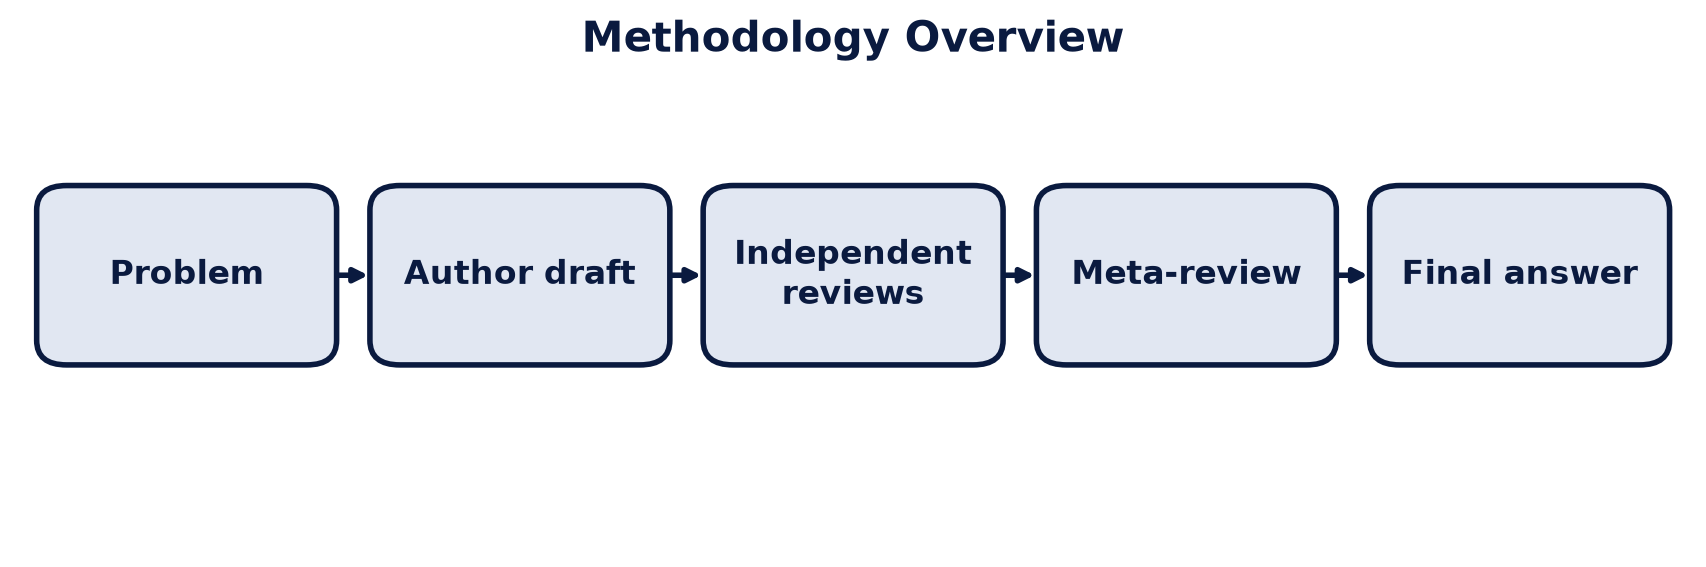
\includegraphics[width=0.9\textwidth,height=0.62\textheight,keepaspectratio]{images/mars_1.png}
\end{center}
\end{frame}

\section{System Architecture}
\begin{frame}{MARS Architecture}
\begin{center}
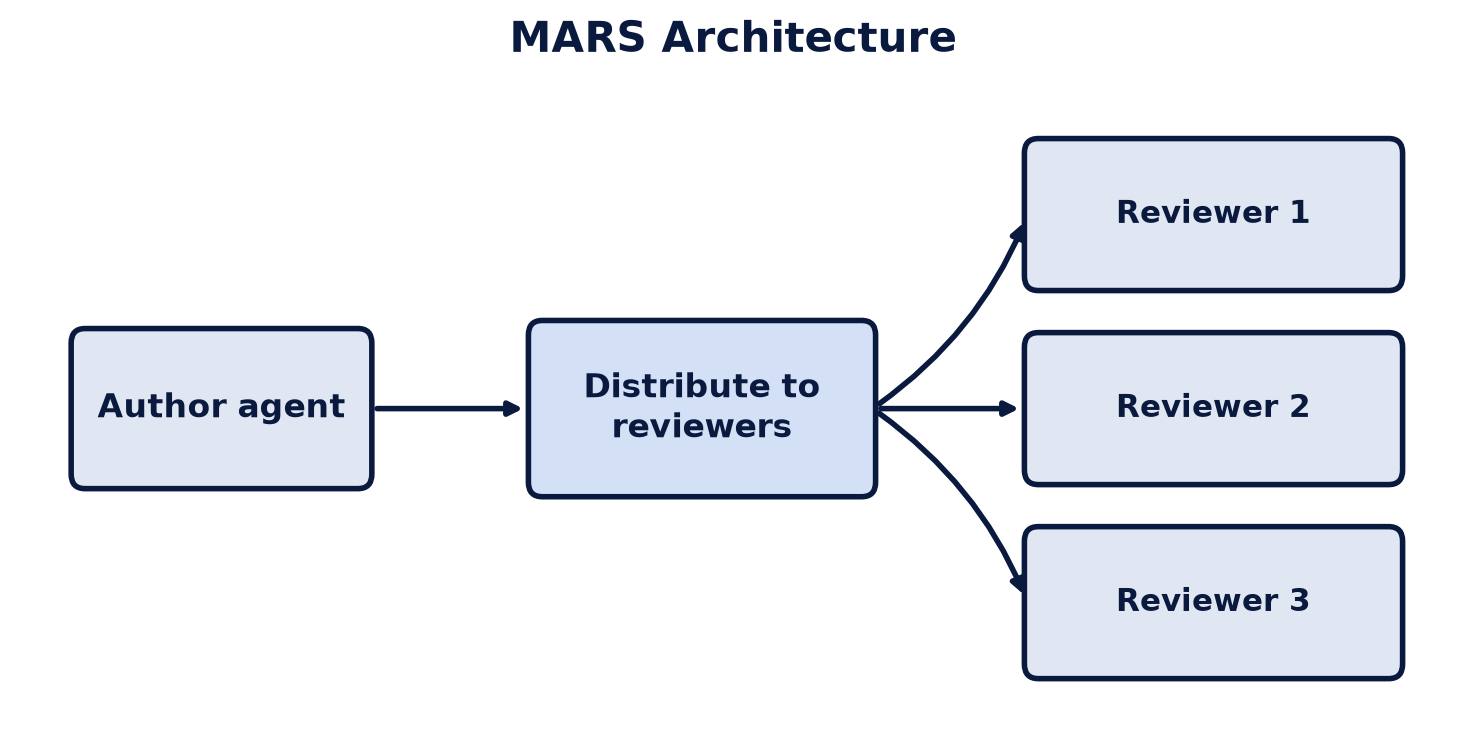
\includegraphics[width=0.9\textwidth,height=0.62\textheight,keepaspectratio]{images/mars_2.png}
\end{center}
\end{frame}

\begin{frame}{Components}
\begin{itemize}
\item \textbf{Author agent:} produces the initial solution.
\item \textbf{Reviewer agents:} independent decisions and comments.
\item \textbf{Meta-reviewer:} integrates, decides, and guides revision.
\item No reviewer-to-reviewer edges, cutting cost.
\end{itemize}
\end{frame}

\section{Data Collection}
\begin{frame}{Benchmarks and Backbones}
\textbf{\textit{Reasoning benchmarks}}
\begin{itemize}
\item \textbf{MMLU:} multi-subject multiple-choice questions.
\item \textbf{GPQA:} graduate biology, physics, chemistry.
\item \textbf{GSM8K:} grade-school math word problems.
\end{itemize}
\textbf{\textit{Model backbones}}
\begin{itemize}
\item Closed: GPT-3.5-turbo, GPT-4o-mini.
\item Open: Mixtral-8x7B, Mixtral-8x22B, Llama3.3-70B.
\end{itemize}
\end{frame}

\section{Model Development}
\begin{frame}{The Review-and-Revision Loop}
\begin{itemize}
\item Author produces candidate reasoning and answer.
\item Reviewers score and comment in parallel.
\item Meta-reviewer accepts or requests revision.
\item Loop continues while decision is reject.
\item Revision rounds capped at two (compute limit).
\end{itemize}
\end{frame}

\section{Results}
\begin{frame}{Accuracy and Efficiency}
\textbf{\textit{Matches MAD accuracy}}
\begin{itemize}
\item GPQA, GPT-3.5: MARS 36.33\% vs MAD 31.00\%.
\item GSM8K, Mixtral-8x22B: 90.33\% vs 87.00\%.
\item GSM8K, GPT-4o-mini: 98.00\% vs 97.67\%.
\end{itemize}
\textbf{\textit{At much lower cost}}
\begin{itemize}
\item Tokens and inference time cut about 50\%.
\end{itemize}
\end{frame}

\begin{frame}{Token Usage per Query}
\begin{center}
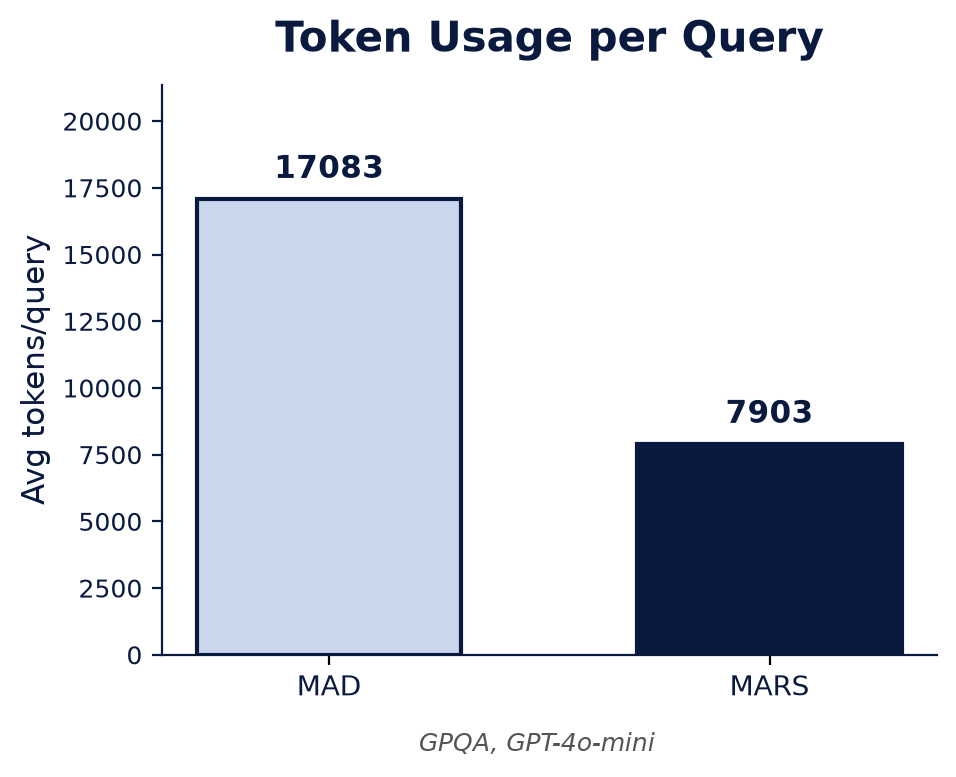
\includegraphics[width=0.9\textwidth,height=0.62\textheight,keepaspectratio]{images/mars_3.png}
\end{center}
\end{frame}

\section{Discussions}
\begin{frame}{Why MARS Works}
\begin{itemize}
\item Independent reviews avoid redundant debate traffic.
\item Efficiency gained without sacrificing accuracy.
\item On hard GPQA, MARS can exceed MAD.
\item Persona assignment gave little to no gain.
\end{itemize}
\end{frame}

\section{Challenges}
\begin{frame}{Limitations}
\begin{itemize}
\item Confidence from token probabilities remains unreliable.
\item Over-correction can overturn correct answers.
\item Revision limited to two rounds by compute.
\item Benefits depend on reviewer quality.
\end{itemize}
\end{frame}

\section{Future Work}
\begin{frame}{Directions Ahead}
\begin{itemize}
\item Study more revision rounds systematically.
\item Design better confidence and stopping criteria.
\item Mitigate over-correction of correct answers.
\item Adapt reviewer count to task difficulty.
\end{itemize}
\end{frame}

\section{Conclusion}
\begin{frame}{Conclusion}
\begin{itemize}
\item MARS reframes collaboration as academic peer review.
\item Author, independent reviewers, and a meta-reviewer.
\item Matches debate accuracy at about half the cost.
\item Efficient, scalable multi-agent reasoning for LLMs.
\end{itemize}
\end{frame}

\section{References}
\begin{frame}{References}
\footnotesize
\begin{itemize}
\item X. Wang, J. Wang, Y. Wang, et al., ``MARS: toward more efficient multi-agent collaboration for LLM reasoning,'' arXiv:2509.20502, 2025.
\item Y. Du, S. Li, A. Torralba, J. B. Tenenbaum, and I. Mordatch, ``Improving Factuality and Reasoning in Language Models through Multiagent Debate,'' arXiv:2305.14325, 2023.
\item J. Wei, X. Wang, D. Schuurmans, et al., ``Chain-of-Thought Prompting Elicits Reasoning in Large Language Models,'' in Proc. NeurIPS, 2022.
\end{itemize}
\end{frame}
\begin{frame}\vfill\centering{\Huge Thank You}\vfill\end{frame}
\end{document}
